\chapter{DG for Elliptic Problem}

First we consider a time-independent elliptic problem. Not only is it
useful for initiation to the subject to first consider a simpler elliptic problem, but it
is also an essential preparational step in deriving the SIPG bilinear form for the
elliptic part of the hyperbolic problem as well.
\\
The goal of this chapter is to build all the necessary theoretical and practical
tools to solve a given elliptic problem
numerically and then experimentally test the method for different parameters.
We will define the necessary notation and derive
the SIPG variational formulation as well as in detail describe further implementation steps as
for example what basis of the finite element space we chose and how to derive local matrices.
Finally this chapter will also include some well established theoretical results in
the context of discontinuous Galerkin methods.
The derivation
of the bilinear form is inspired by
Chapter 1 in \cite{riviere2008} as well as \cite{georgoulis2011Springer} and \cite{grote2006}
for cross reference.

%---Problem---------------------------------------------------------------
\section{Problem}
We consider the following elliptic model problem:
\begin{equation}
	\label{eq:elliptic_pde}
	-(c(x)u'(x))' = f(x) \qquad \forall x\in \Omega
\end{equation}
\begin{equation}
	\label{eq:elliptic_pde_bc}
	u(0) = g_0, u(1) = g_1
\end{equation}
where $\Omega = (0,1)$ is the domain, $g_0, g_1 \in \mathbb{R}$ are
Dirichlet boundary conditions, $f \in L^2(\Omega)$ and $c:\Omega \to \mathbb{R}$
satisfies:
\[
	c_{\min} \leq c(x) \leq c_{\max} \qquad \forall x\in \Omega
\]
for $0 < c_{\min} \leq c_{\max}$.
Multiplying the solution by a test function and integrating by parts over $\Omega$ we get the
standard weak formulation: \\
Find $u \in H^1(\Omega)$ such that:
\begin{equation}
	a(u,v) = (f,v)_{L^2(\Omega)} \qquad \forall v \in C_c^{\infty}(\Omega)
\end{equation}
Where
\[
	a:H^1(\Omega) \times H^1(\Omega) \to \mathbb{R}, \qquad (u,v) \mapsto \int_{\Omega} c(x)u'(x)v'(x) \text{d}x
\]
defines the standard elliptic bilinear form on $H^1(\Omega)$ and
\[
	(u,v)_{L^2(\Omega)} = \int_{\Omega} uv \,\text{d}x
\]

denotes the $L^2$-inner product.

%---Discretization---------------------------------------------------------
\section{Discretization}
Let $0=x_0 < \cdots < x_{N+1} = 1$ be the mesh faces, $I_n = (x_n, x_{n+1})$ for $n = 0,\ldots,N$ be the elements and $\mathcal{T}_h = \{I_n\}_{n=0}^N$ a partition
of $\Omega$ for some fixed $N\in \mathbb{N}$.
We denote the element length by $h_n = x_{n+1} - x_{n}$ for $n=0,\ldots,N$ and the global meshsize by
$h = \max_{n} h_n$.
Next we define the discontinuous finite element space
\begin{tcolorbox}[mythmstyle, colback=green!10!white]
	\begin{equation}
		V_h^r(\mathcal{T}_h) = \{v \in L^2(\Omega) |\, v|_{I_n} \in \mathcal{P}^r(I_n) \}
	\end{equation}
\end{tcolorbox}
where $\mathcal{P}^r(I_n)$ denotes the space of polynomials $p:I_n \to \mathbb{R}$ of degree $r$
for $r \in \mathbb{N}$. When the context allows it, we will denote the
finite element space with just $V_h$ for simplicity.
$V_h$ is our final approximation space in which the numerical solution
lays.
We observe that in contrast to a continuous finite element approximation space
here the resulting solution is a priori discontinuous by construction.
Furthermore we have here $V_h \not\subset H^1(\Omega)$.
This is especially apparent in 1d due to the Sobolev embedding $H^1(\Omega) \subset C^0(\Omega)$.
Any discontinuous element of $V_h$ can therefore not be in $H^1(\Omega)$. \\
To proceed we will require the following trace operators:

\begin{definition}
	\label{def:jump_average}
	Let $v:\Omega \to \mathbb{R}$ be piecewise continuous and let $n \in
		\{1,\ldots,N\}$
	\begin{enumerate}[label=\textnormal{(\roman*)}]
		\item We denote $v(x_n^+) := \lim_{x \searrow x_n} v(x), v(x_n^-) := \lim_{x \nearrow x_n} v(x)$
		      the limit from above/below.
		\item We define the \textbf{jump} at $x_n$ as
		      \[
			      [v(x_n)]:= v(x_n^-) - v(x_n^+)
		      \]
		      and the \textbf{average} at $x_n$ as
		      \[
			      \{v(x_n)\}:= \frac{v(x_n^+) + v(x_n^-)}{2}
		      \]
		      furthermore by convention we set:
		      \[
			      [v(x_0)] := -v(x_0^+),\quad [v(x_{N+1})] := v(x_{N+1}^-),\quad
			      \{v(x_0)\}:=v(x_0^+),\quad \{v(x_{N+1})\}:= v(x_{N+1}^-)
		      \]
	\end{enumerate}
\end{definition}

%---Variational Formulation--------------------------------------------------------
\section{Variational Formulation}
To derive the SIPG variational formulation, let $v \in V_h$ be a test
function. For simplicity suppose for now that the coefficient $c \in C^1(\Omega)$ and
the exact solution $u \in H^2(\Omega) \subset C^1(\Omega)$.
Due to the discontinuity of the test function in contrast to
continuous FEM we multiply $u$ with $v$ on each element $I_n$
and integrate by parts locally
\begin{equation*}
	\int_{x_n}^{x_{n+1}} fv\, \text{d}x = -\int_{x_n}^{x_{n+1}} (cu')'v\, \text{d}x
	= \int_{x_n}^{x_{n+1}} cu'v'\, \text{d}x
	-  cu'v\Big|_{x_n}^{x_{n+1}} \qquad \forall n=0,\ldots,N
\end{equation*}
then sum over all elements
\begin{equation}
	\label{eq:elliptic_sipg_var_form_incomplete}
	(f,v)_{L^2(\Omega)} = \sum_{n=0}^N \int_{I_n} cu'v'\, \text{d}x
	-\sum_{n=0}^{N+1} [c(x_n)u'(x_n)v(x_n)]
\end{equation}
where we have used that $\sum_{n=0}^N  w \Big|_{x_n}^{x_{n+1}} = w(x_{N+1}^-) -
	w(x_{N}^+) + w(x_{N}^-) - \cdots - w(x_1^+) + w(x_1^-) - w(x_0^+) = \sum_{n=0}^{N+1} [w(x_n)]$ for any piece-wise continuous function $w$.
\\
By our construction are $c, u'$ continuous on $\Omega$, this means
\begin{equation}
	\label{eq:id_1_cu_jump_zero}
	[c(x_n)u'(x_n)v(x_n)] = c(x_n)u'(x_n)[v(x_n)] = \{c(x_n)u'(x_n)\}[v(x_n)] \qquad \forall n=0,\ldots,N+1
\end{equation}
and
\begin{equation}
	\label{eq:id_2_u_jump_zero}
	[u(x_n)] = 0 \qquad \forall n=1,\ldots,N
\end{equation}
To derive the final variational form we will now have to add two additional terms
to (\ref{eq:elliptic_sipg_var_form_incomplete}): \\
\textbf{Step 1.} Firstly we need to symmetrize our currently non-symmetrical right hand side
which will correspond to the SIPG bilinear form. To do so
we subtract $\sum_{n=0}^{N+1} \{c(x_n)v'(x_n)\}[u(x_n)]$ on both sides of
(\ref{eq:elliptic_sipg_var_form_incomplete}) so we get
\begin{align*}
	  & (f,v)_{L^2(\Omega)}-g_1c(x_{N+1}^-)v(x_{N+1}^-) + g_0c(x_0^+)v(x_0^+) \\
	= & \sum_{n=0}^N \int_{I_n} cu'v'\, \text{d}x
	-\sum_{n=0}^{N+1} \{c(x_n)u'(x_n)\}[v(x_n)] + \{c(x_n)v'(x_n)\}[u(x_n)]
\end{align*}
where on the left hand side of the equation we have applied (\ref{eq:id_2_u_jump_zero})
for the interior node contributions of the sum (which therefore vanish), and the boundary condition (\ref{eq:elliptic_pde_bc})
ensuring the left hand side to be soley dependent on $v$.\\
\textbf{Step 2.} The bilinear form we seek to create will (for now) be defined on $V_h\times V_h$
meaning it will intake discontinuous functions. In particular the numerical
solution will be a discontinuous function wheras the exact solution is continuous.
To counterweigh this discrepancy we need to integrate a penalization mechanism, seeking to
minimize discontinuous behaviors. Technically speaking this penalization term
will guarantee coercivity of the bilinear form (see section \ref{sec:existence_uniqueness_elliptic_discrete_problem}). \\
Let $\sigma > 0$ constant, we define:
\begin{equation*}
	\texttt{c}_n :=
	\begin{cases}
		\max(c(x_n^+), c(x_n^-)), & n=1,\ldots,N \\
		c(x_n^+),                 & n=0          \\
		c(x_n^-),                 & n=N+1
	\end{cases},
	\qquad \texttt{h}_n :=
	\begin{cases}
		\min(h_n, h_{n-1}), & n=1,\ldots,N    \\
		h_n,                & n\in \{0, N+1\}
	\end{cases}
\end{equation*}
with this we define our penalization parameter
\begin{tcolorbox}[mythmstyle, colback=green!10!white]
	\begin{equation}
		\label{def:penalization_function}
		\texttt{a}_n := \frac{\sigma \texttt{c}_n}{\texttt{h}_n} > 0 \qquad \forall n=0\ldots,N+1
	\end{equation}
\end{tcolorbox}
Similarly to Step 1 we can now add the term $\sum_{n=0}^{N+1} \texttt{a}_n[u(x_n)][v(x_n)]$
on both sides of (\ref{eq:elliptic_sipg_var_form_incomplete}) and get the final
\textit{discrete} SIPG variational formulation.\\
\begin{tcolorbox}[mythmstyle, colback=green!10!white]
	Find $u_h \in V_h$ such that:
	\begin{equation}
		\label{eq:discrete_var_form_elliptic}
		b_h(u_h, v) = \ell(v), \qquad \forall v\in V_h
	\end{equation}
	where
	\begin{align*}
		b_h(u,v) & = \sum_{n=0}^N \int_{I_n} cu'v'\, \text{d}x
		-\sum_{n=0}^{N+1} \{c(x_n)u'(x_n)\}[v(x_n)] + \{c(x_n)v'(x_n)\}[u(x_n)]
		+\sum_{n=0}^{N+1} \texttt{a}_n[u(x_n)][v(x_n)]                                     \\
		\ell(v)  & = (f,v)_{L^2(\Omega)}-g_1c(x_{N+1}^-)v(x_{N+1}^-) + g_0c(x_0^+)v(x_0^+)
		+ \texttt{a}_{N+1}g_1v(x_{N+1}^-) + \texttt{a}_0 g_0v(x_{0}^+)
	\end{align*}
	for $u,v\in V_h$.
\end{tcolorbox}

%---Boundary Conditions----------------------------------------------------------
\section{Boundary Conditions}
By adding the terms $-\sum_{n=0}^{N+1} \{c(x_n)v'(x_n)\}[u(x_n)], \sum_{n=0}^{N+1} \texttt{a}_n[u(x_n)][v(x_n)]$ on both sides
of (\ref{eq:elliptic_sipg_var_form_incomplete}) we \textit{weakly} imposed the Dirichlet
boundary conditions into the variational form. This stands in contrast to how boundary
conditions are usually imposed in continuous FEM. Indeed one could also impose them strongly,
meaning we could define
\begin{equation*}
	V_h^r(\mathcal{T}_h) = \{v \in L^2(\Omega) |\, v|_{I_n} \in \mathcal{P}^r(I_n), v(x_0)=g_0, v(x_{N+1})=g_1 \}
\end{equation*}
but this soley as a side note, we will continue to work with purely weakly imposed
boundary conditions.  \\ \\

One could alternatively desire to implement \textit{Neumann} boundary conditions, this slightly changes the variational formulation.
We illustrate the idea on the following example boundary condition. A solution
$u$ should satisfy:
\[
	u(0) = g_{0}, u'(1)\cdot n_1 = g_{1}
\]
where again $g_0, g_1 \in \mathbb{R}$ are the boundary values and $n_1$ denotes the outward normal
of the domain at the upper boundary. In 1d we trivially have $n_1 = 1, n_0 = -1$, where $n_0$ denotes the outward
normal at the lower boundary.

Now recall the initial incomplete formulation (\ref{eq:elliptic_sipg_var_form_incomplete}). First we take the
Neumann boundary contribution $\{c(x_{N+1})u'(x_{N+1})\}[v(x_{N+1})]$ to the other side of the equation. We get
\[
	\sum_{n=0}^N \int_{I_n} cu'v'\, \text{d}x
	-\sum_{n=0}^{N} \{c(x_n)u'(x_n)\}[v(x_n)] = (f,v)_{L^2(\Omega)}
	+ g_1c(x_{N+1}^-)v(x_{N+1}^-)
\]
We have used $\{c(x_{N+1})u'(x_{N+1})\}[v(x_{N+1})] = c(x_{N+1}^-)u'(x_{N+1}^-)v(x_{N+1}^-)\cdot n_1 = g_1 c(x_{N+1}^-)v(x_{N+1}^-)$

From here on
we proceed similarly as in the Dirichlet case. The main difference is that we always ommit the boundary face with the Neumann
boundary condition. \\
We add the terms
\[
	-\sum_{n=0}^{N} \{c(x_n)v'(x_n)\}[u(x_n)]
	+\sum_{n=0}^{N} \texttt{a}_n[u(x_n)][v(x_n)]
\]
to both sides, using again that the real solution has zero jump on the interior faces and
applying the boundary conditions we finally derive the variational form

\begin{align*}
	 & \sum_{n=0}^N \int_{I_n} cu'v'\, \text{d}x
	-\sum_{n=0}^{N} \{c(x_n)u'(x_n)\}[v(x_n)] + \{c(x_n)v'(x_n)\}[u(x_n)]
	+\sum_{n=0}^{N} \texttt{a}_n[u(x_n)][v(x_n)]                                \\
	 & = (f,v)_{L^2(\Omega)} + g_0c(x_0^+)v(x_0^+) + \texttt{a}_0 g_0v(x_{0}^+)
	+ g_1c(x_{N+1}^-)v(x_{N+1}^-)
\end{align*}


%---Matrix-Vector System---------------------------------------------------------
\section{Matrix-Vector System}
We will now in derive the fully discrete Matrix-Vector system given by
the variational form (\ref{eq:discrete_var_form_elliptic}). To do so let
$r \in \mathbb{N}$ denote the polynomial degree and consequently the element degree of freedom.
Note that in this thesis we will only consider global polynomial degrees, meaning one set polynomial degree for all elements.
Next let $\{\Phi_0,\ldots,\Phi_M\}$ be a basis of $V_h$, where $M = \dim(V_h)$.
We can represent the sought Galerkin approximation as $u_h = \sum_{j=0}^{M} \alpha_j \Phi_j\in V_h$ for coefficients
$\alpha_j \in \mathbb{R}$. Then (\ref{eq:discrete_var_form_elliptic}) is equivalent to:
\begin{equation*}
	\sum_{j=0}^{M} \alpha_j b_h(\Phi_j, \Phi_i) = \ell(\Phi_i) \qquad \forall i=0,\ldots,M
\end{equation*}
which corresponds to the system:
\begin{equation}
	\label{eq:fully_discrete_dg_system_elliptic}
	\textbf{Bu} = \textbf{l}
\end{equation}
for $ \textbf{B} \in \mathbb{R}^{M\times M}, [\textbf{B}]_{i,j} = b_h(\Phi_j, \Phi_i),
	\textbf{u} \in \mathbb{R}^M, [\textbf{u}]_j = \alpha_j,
	\textbf{l}\in\mathbb{R}^M, [\textbf{l}]_j = \ell(\Phi_j)$.

%---Basis-of-FE-Space------------------------------------------------------------
\section{Basis of Finite Element Space}
\label{sec:ell_basis}
There are many ways of choosing basis functions for finite element spaces. We choose a Lagrangian
nodal elementwise basis where the nodes per element correspond to the Gauss-Lobatto quadrature nodes.
This is a commonly used nodal basis in continuous 1d-FEM and we will also use it for our DG method. In Appendix A.2.3 of \cite{diPietro2012} the \textit{Fekete points} are recommended 
with the argument that this nodal basis yields a mass matrix with optimal an condition number. In 1d the Fekete points coincide with the Gauss-Lobatto quadrature nodes. 
One could fill an entire chapter with the discussion on the choice of basis functions, so 
we will not go into any detail here but note the following, when assembling mass and stiffness matrices we have to approximate a integral, so the question of choosing a fitting quadrature 
rule arises. If we choose the same nodes for the quadrature as for the basis, i.e. use the Gauss-Lobatto quadrature rule we have to take into account that this quadrature for $r+1$ points 
is only exact for polynomials of degree $2r-1$. \\ 
If we assume a piecewise constant coefficient $c$, we calculate the integral in the assembly of the stiffness matrix exactly since
for $\mathcal{P}^r$-elements we have $r+1$ basis (and quadrature) nodes and the to be approximated integral is of the form
$ c_I \int_I \Phi_j^{\prime} \Phi_i^{\prime} \text{d}x $ where $I \in \mathcal{T}_h$ is a element and $\Phi_i \vert_I, \Phi_j \vert_I \in \mathcal{P}^r(I)$ are basis functions, where
$ \Phi_j^{\prime} \Phi_i^{\prime} \in \mathcal{P}^{2r-2}$.
In contrast if we intend to approximate for the mass matrix, which is of the form $ \int_I \Phi_j \Phi_i \text{d}x $ we will introduce an error, since $ \Phi_j \Phi_i \in \mathcal{P}^{2r}$.
 
For more detailed information on choosing basis functions and alternative approaches see for example
Appendix A.2 in \cite{diPietro2012}. \\ \\
Let $n\in \{1,\ldots,N\}$ and $I_n \in \mathcal{T}_h$ be an arbitrary element.
We denote $\hat{I} = (-1,1)$ the \textit{reference element} and $\displaystyle F_n : \hat{I} \to I_n, \, \xi \mapsto \frac{x_n + x_{n+1}}{2} + \frac{h_n}{2} \xi $
the \textit{element map}. This now allows us to define a basis on the reference element and
extend it to all elements using the element map. \\
For a fixed polynomial degree $r \geq 2$ let $\xi_0,\ldots,\xi_{r} \in [-1,1]$ be the
Gauss-Lobatto nodes. \\
\begin{equation*}
	\begin{tabular}{c|c}
		\centering
		$r = 2$ & $\{-1, 1\}$                                         \\
		$r = 3$ & $\{-1,0, 1\}$                                       \\
		$r = 4$ & $\{-1,-\frac{1}{\sqrt{5}}, \frac{1}{\sqrt{5}}, 1\}$ \\
		\vdots  & \vdots                                              \\
	\end{tabular}
\end{equation*}
The inner nodes are given by the roots of $L_{r-1}^{\prime}$, the derivative of the $r-1$-th Legendre polynomial.
We define the basis on the reference element as the Lagrangian nodal basis

\begin{equation}
	\label{def:lagrange_ref_basis}
	\widehat{\phi}_i(\xi) := \prod_{\substack{j = 0 \\ j\neq i}}^{r}\frac{\xi - \xi_j}{\xi_i - \xi_j},
	\qquad \text{for } i=0,\ldots,r
\end{equation}
and define the basis functions on the element $I_n$ as
\begin{equation}
	\phi^n_i : I_n \to \mathbb{R}, \quad \phi^n_i(x) := \widehat{\phi}_i(F_n^{-1}(x))
	\nonumber
\end{equation}
as a last step we extend the basis functions to the whole domain $\Omega$ by zero
\begin{equation}
	\Phi_i^n: \Omega \to \mathbb{R}, \quad \Phi_i^n(x) :=
	\begin{cases}
		\phi_i^n(x), & \text{for } x\in I_n \\
		0,           & \text{else}
	\end{cases}
	\label{def:lagrange_basis_of_Vh}
\end{equation}
for $n=0,\ldots,N$ and $i=0,\ldots,r$. Clearly we have $\text{span}( \widehat{\phi}_0, \ldots, \widehat{\phi}_r) = \mathcal{P}^r(\hat{I})$
and by extension $\text{span}(\Phi_0^0,\ldots,\Phi_r^N) = V_h^r(\mathcal{T}_h)$. It is essential
that our basis has only local support, meaning the basis functions are zero on most of the domain. This is the key property which
allows the final matrices to be sparse. Choosing basis functions with global support, the computational cost would be unfeasible for
small mesh sizes. \\
By having chosen a Lagrangian nodal basis the mesh nodes exactly coincide with the Gauss-Lobatto nodes on each
element.
To simplify the notation we introduce a \textit{local-to-global} index map
\begin{equation}
	\label{def:local_to_global_map}
	T: \{0,\ldots,N\} \times \{0,\ldots,r\} \to \{1,\ldots,M\}
\end{equation}
where $M = (r+1)(N+1) = \dim(V_h)$. $T$ takes an element index $n$ and a local basis function index $i$ as inputs
and returns the globally assigned node index $T(n,i)$. $T$ corresponds to the
\textit{connectivity matrix}. In the simplest case we have the global index ordered from left to right and get
$T(n,i) = nr + i$.


%---Matrix Assembly-------------------------------------------------------------------
\section{System Matrix Assembly}
With the basis functions in (\ref{def:lagrange_basis_of_Vh}) defined we can now in detail investigate how
to assemble the matrix $\textbf{B}$ in (\ref{eq:fully_discrete_dg_system_elliptic}). To do so we firstly separate
the bilinear form $b_h$ into different components

\begin{align*}
	a_h(u,v)                & := \sum_{n=0}^N \int_{I_n} cu'v'\, \text{d}x                              \\
	b_h^{\text{cons}}(u,v)  & := \sum_{n=0}^{N+1} \{c(x_n)u'(x_n)\}[v(x_n)] + \{c(x_n)v'(x_n)\}[u(x_n)] \\
	b_h^{\text{penal}}(u,v) & := \sum_{n=0}^{N+1} \texttt{a}_n[u(x_n)][v(x_n)]                          \\
\end{align*}

Let $\displaystyle u_h = \sum_{m=0}^{N} \sum_{j=0}^{r} \alpha_j^m \Phi_j^m \in V_h$ denote
the Galerkin approximation, then as discussed in section \ref{sec:ell_basis} the discrete variational formulation (\ref{eq:discrete_var_form_elliptic}) is equivalent
to
\begin{equation}
	\sum_{m=0}^{N} \sum_{j=0}^{r} \alpha_j^m \Big(
	a_h(\Phi_j^m,\Phi_i^n) - b_h^{\text{cons}}(\Phi_j^m,\Phi_i^n) + b_h^{\text{penal}}(\Phi_j^m,\Phi_i^n)
	\Big)
	= \ell(\Phi_i^n), \qquad \forall n=0,\ldots,N, i=0,\ldots,r
\end{equation}
which corresponds to the matrix vector system (\ref{eq:fully_discrete_dg_system_elliptic})
where we can write
\begin{equation*}
	\textbf{B} = \textbf{A} - \textbf{B}_{\text{cons}} + \textbf{B}_{\text{penal}}
\end{equation*}
we will assemble the three (symmetric) matrices separately.
\begin{align*}
	 & [\textbf{B}]_{T(n,i),T(m,j)} = b_h(\Phi_j^m, \Phi_i^n),
	 & [\textbf{A}]_{T(n,i),T(m,j)} = a_h(\Phi_j^m, \Phi_i^n)                                \\
	 & [\textbf{B}_{\text{cons}}]_{T(n,i),T(m,j)} = b_h^{\text{cons}} (\Phi_j^m, \Phi_i^n)
	 & [\textbf{B}_{\text{penal}}]_{T(n,i),T(m,j)} = b_h^{\text{penal}} (\Phi_j^m, \Phi_i^n)
\end{align*}
where $T$ is given by (\ref{def:local_to_global_map})

\subsection{Assembly of A}
$\textbf{A}$ is assembled exactly as the standard stiffness matrix in continuous finite element.
We can rewrite $\textbf{A} = \sum_{s=0}^{N} \textbf{A}^{(s)}$, where
$[\textbf{A}^{(s)}]_{T(n,i),T(m,j)} = \int_{I_s} c \,(\Phi_j^m)' (\Phi_i^n)' \, \text{d}x$.
Now since we have $\text{supp}(\Phi_i^n)\subset I_n$ the only non-zero entries of $\textbf{A}^{(s)} $ are the ones where both $n=m=s$. Pulling back the integral
to the reference element using the chain rule and the substitution $F_s^{-1}(x) = \xi$ we find
\begin{equation*}
	\int_{I_s} c(x) \,(\Phi_j^s)'(x) (\Phi_i^s)'(x) \, \text{d}x =
	\frac{2}{h_s} \int_{\hat{I}} c(F_s(\xi)) \, \widehat{\phi}_j^{\, \prime}(\xi) \widehat{\phi}_i^{\, \prime}(\xi) \, \text{d}\xi
\end{equation*}
This integral now only depends on the reference shape functions, the element length $h_s$
and the values of the coefficient $c$. Using the Gauss-Lobatto quadrature rule we can approximate the integral
only requiring the values of $c$ at the nodes, whilst having the values of $\phi, \phi'$ preloaded.
The total assembly of $\textbf{A}$ can therefore be achieved by calculating a local contribution matrix
$\widehat{\textbf{A}}^{(s)} \in \mathbb{R}^{(r+1)\times (r+1)}$ for each element $I_s$ and adding it into $\textbf{A}$.
\begin{example}
	For $c\equiv 1$ with $\mathcal{P}^1$-elements $(r=1)$ we have
	\begin{equation*}
		\widehat{\textbf{A}}^{(s)} = \frac{1}{h_s}
		\begin{bmatrix}
			1  & -1 \\
			-1 & 1
		\end{bmatrix}
	\end{equation*}
\end{example}

\subsection{Assembly of B consistency part}
\label{subsec:assembly_cons}
As before we rewrite $\textbf{B}_{\text{cons}} = \sum_{s=0}^{N+1} \textbf{B}_{\text{cons}}^{(s)} $, where

\begin{equation*}
	[\textbf{B}_{\text{cons}}^{(s)}]_{T(n,i),T(m,j)} = \{c(x_s) \Phi_j^{m \, \prime} (x_s)\}[\Phi_i^n(x_s)] + \{c(x_s)\Phi_i^{n\, \prime} (x_s)\}[\Phi_j^m(x_s)]
\end{equation*}

\subsubsection{Interior Faces}
First let $s \in \{1,\ldots,N\}$ denote an interior face, we observe again, that the entries of
$\textbf{B}_{\text{cons}}^{(s)}$ can only be non-zero for an index tuple $(T(n,i),T(m,j))$ if
$n,m \in \{s, s-1\}$ by the local support of the basis functions.
Therefore assembling $ \textbf{B}_{\text{cons}}$ again comes down to calculating a local contribution matrix

\begin{equation*}
	\widehat{\textbf{B}}_{\text{cons}}^{(s)} =
	\begin{bmatrix}
		\textbf{C}_{\text{cons}}^{(s-1,s-1)} & \textbf{C}_{\text{cons}}^{(s-1,s)} \\
		\textbf{C}_{\text{cons}}^{(s,s-1)}   & \textbf{C}_{\text{cons}}^{(s,s)}
	\end{bmatrix}
	\in \mathbb{R}^{2(r+1) \times 2(r+1)}
\end{equation*}
for each interior face $x_s$ consisting of four blocks we will now lay out in more detail.
We discuss the boundary case separately.
Using again the local support of the basis functions we find
\begin{align*}
	 & [\textbf{C}_{\text{cons}}^{(s-1,s-1)}]_{i,j} = \frac{c(x_s^-)}{2} \Phi_j^{s-1\, \prime}(x_s^-) \Phi_i^{s-1}(x_s^-) + \frac{c(x_s^-)}{2} \Phi_i^{s-1\, \prime}(x_s^-) \Phi_j^{s-1}(x_s^-) \\
	 & [\textbf{C}_{\text{cons}}^{(s-1,s)}]_{i,j} = \frac{c(x_s^+)}{2} \Phi_j^{s\, \prime}(x_s^+) \Phi_i^{s-1}(x_s^-) - \frac{c(x_s^-)}{2} \Phi_i^{s-1\, \prime}(x_s^-) \Phi_j^{s}(x_s^+)       \\
	 & [\textbf{C}_{\text{cons}}^{(s,s)}]_{i,j} = -\frac{c(x_s^+)}{2} \Phi_j^{s\, \prime}(x_s^+) \Phi_i^{s}(x_s^+) - \frac{c(x_s^+)}{2} \Phi_i^{s\, \prime}(x_s^+) \Phi_j^{s}(x_s^+)
\end{align*}
where we have used the definitions of jump and average in (\ref{def:jump_average}).
Note that $ \textbf{C}_{\text{cons}}^{(s-1,s)} = (\textbf{C}_{\text{cons}}^{(s,s-1)})^T$ by the symmetry of the bilinear form $b_h^{\text{cons}}$.
Next we represent the values of the basis functions $ \Phi $ at the element boundary by the values of the reference
shape functions $\widehat{\phi}$
\begin{align}
	 & \Phi_i^s(x_s^+) = \widehat{\phi}_i(-1) ,                                                   & \Phi^{s-1}_i(x_s^-) = \widehat{\phi}_i(1) \label{eq:shape_fun_and_basis_fun_values_equality} \\
	 & \Phi_i^{s\, \prime }(x_s^+) = \frac{2}{h_{s}} \widehat{\phi}_i^{\,\prime}(-1),
	 & \Phi_i^{s-1\, \prime }(x_s^-) = \frac{2}{h_{s-1}} \widehat{\phi}_i^{\,\prime}(1) \nonumber
\end{align}
which finally yields
\begin{align*}
	 & [\textbf{C}_{\text{cons}}^{(s-1,s-1)}]_{i,j} = \frac{c(x_s^-)}{h_{s-1}} \widehat{\phi}_j^{\,\prime}(1) \widehat{\phi}_i(1) + \frac{c(x_s^-)}{h_{s-1}} \widehat{\phi}_i^{\,\prime} (1) \widehat{\phi}_j(1)  \\
	 & [\textbf{C}_{\text{cons}}^{(s-1,s)}]_{i,j} = \frac{c(x_s^+)}{h_{s}} \widehat{\phi}_j^{\,\prime} (-1) \widehat{\phi}_i (1) - \frac{c(x_s^-)}{h_{s-1}} \widehat{\phi}_i^{\,\prime} (1) \widehat{\phi}_j (-1) \\
	 & [\textbf{C}_{\text{cons}}^{(s,s)}]_{i,j} = -\frac{c(x_s^+)}{h_s} \widehat{\phi}_j^{\,\prime} (-1) \widehat{\phi}_i (-1) - \frac{c(x_s^+)}{h_s} \widehat{\phi}_i^{\,\prime} (-1) \widehat{\phi}_j (-1)
\end{align*}
\begin{example}
	Consider $c\equiv 1$ for $\mathcal{P}^1$-elements $(r=1)$
	with an equidistant mesh with meshsize $h$ we have
	\begin{equation*}
		\widehat{\textbf{B}}_{\text{cons}}^{(s)} = \frac{1}{h}
		\begin{bmatrix}
			0    & -1/2 & 1/2  & 0    \\
			-1/2 & 1    & -1   & 1/2  \\
			1/2  & -1   & 1    & -1/2 \\
			0    & 1/2  & -1/2 & 0
		\end{bmatrix}
	\end{equation*}
\end{example}

\subsubsection{Boundary Faces}
For $s\in \{0, N+1 \}$ and $x_s$ a boundary face we now have a smaller local contribution matrix
since the contribution can only come from the one element to which $x_s$ belongs. Meaning we have
$\widehat{\textbf{B}}_{\text{cons}}^{(0)}, \widehat{\textbf{B}}_{\text{cons}}^{(N+1)} \in \mathbb{R}^{(r+1)\times (r+1)}$
with
\begin{align*}
	 & [\widehat{\textbf{B}}_{\text{cons}}^{(0)}]_{i,j} =
	-\frac{2 c(x_0^+)}{h_{0}} \widehat{\phi}_j^{\,\prime}(-1) \widehat{\phi}_i(-1) - \frac{2 c(x_0^+)}{h_{0}} \widehat{\phi}_i^{\,\prime} (-1) \widehat{\phi}_j(-1)         \\
	 & [\widehat{\textbf{B}}_{\text{cons}}^{(N+1)}]_{i,j} =
	\frac{2 c(x_{N+1}^-)}{h_{N+1}} \widehat{\phi}_j^{\,\prime}(1) \widehat{\phi}_i(1) + \frac{ 2 c(x_{N+1}^-)}{h_{N+1}} \widehat{\phi}_i^{\,\prime} (1) \widehat{\phi}_j(1) \\
\end{align*}

\begin{example}
	For $c\equiv 1$ with $\mathcal{P}^1$-elements $(r=1)$ we have
	\begin{equation*}
		\widehat{\textbf{B}}_{\text{cons}}^{(0)} = \frac{1}{h_0}
		\begin{bmatrix}
			2  & -1 \\
			-1 & 0
		\end{bmatrix}
		,\qquad
		\widehat{\textbf{B}}_{\text{cons}}^{(N+1)} = \frac{1}{h_{N+1}}
		\begin{bmatrix}
			0  & -1 \\
			-1 & 2
		\end{bmatrix}
	\end{equation*}
\end{example}

\subsection{Assembly of B penalty part}
Again we rewrite $\textbf{B}_{\text{penal}} = \sum_{s=0}^{N+1} \textbf{B}_{\text{penal}}^{(s)}$, where
\begin{equation*}
	[\textbf{B}_{\text{penal}}^{(s)}]_{T(n,i), T(m,j)} = { \texttt{a}_s} [\Phi_j^m(x_s)] [\Phi_i^n(x_s)]
\end{equation*}
We proceed analogously to \ref{subsec:assembly_cons}.
\subsubsection{Interior Faces}
Let $s\in \{1,\ldots,N\} $ and $x_s$ denote an interior face. As before we have that
the entries of $ \textbf{B}_{\text{penal}}^{(s)} $ can only be nonzero for an index tuple
$ (T(n,i), T(m,j)) $ if $ n,m \in \{s, s-1\} $, similar to \ref{subsec:assembly_cons} we find
that the assembly boils down to adding up local contributions represented in a local contribution
matrix

\begin{equation*}
	\widehat{\textbf{B}}_{\text{penal}}^{(s)} =
	\begin{bmatrix}
		\textbf{C}_{\text{penal}}^{(s-1,s-1)} & \textbf{C}_{\text{penal}}^{(s-1,s)} \\
		\textbf{C}_{\text{penal}}^{(s,s-1)}   & \textbf{C}_{\text{penal}}^{(s,s)}
	\end{bmatrix}
	\in \mathbb{R}^{2(r+1) \times 2(r+1)}
\end{equation*}

and using (\ref{eq:shape_fun_and_basis_fun_values_equality}), and the definition of the penalization
parameter (\ref{def:penalization_function}) we specifically find

\begin{align*}
	 & [\textbf{C}_{\text{penal}}^{(s-1,s-1)}]_{i,j} = \texttt{a}_s \widehat{\phi}_j(1) \widehat{\phi}_i(1) \\
	 & [\textbf{C}_{\text{penal}}^{(s-1,s)}]_{i,j} = -\texttt{a}_s \widehat{\phi}_j(-1) \widehat{\phi}_i(1) \\
	 & [\textbf{C}_{\text{penal}}^{(s,s)}]_{i,j} = \texttt{a}_s \widehat{\phi}_j(-1) \widehat{\phi}_i(-1)
\end{align*}

where again by symmetry of the penalty term we have
$ \textbf{C}_{\text{penal}}^{(s-1,s)} = (\textbf{C}_{\text{penal}}^{(s,s-1)})^T$
and $\texttt{a}_s$ only depends on the two adjacent elements $I_{s-1}, I_s$.

\begin{example}
	Consider $c\equiv 1$ for $\mathcal{P}^1$-elements $(r=1)$
	with an equidistant mesh with meshsize $h$ we have
	\begin{equation*}
		\widehat{\textbf{B}}_{\text{penal}}^{(s)} = \frac{\sigma}{h}
		\begin{bmatrix}
			0 & 0  & 0  & 0 \\
			0 & 1  & -1 & 0 \\
			0 & -1 & 1  & 0 \\
			0 & 0  & 0  & 0
		\end{bmatrix}
	\end{equation*}
\end{example}

\subsubsection{Boundary Faces}
For $s \in  \{0, N+1\} $ we again have only the respective boundary element contributing.
So the local contribution matrices $ \widehat{\textbf{B}}_{\text{penal}}^{(s)} \in \mathbb{R}^{(r+1) \times (r+1)} $ satisfy

\begin{align*}
	[\widehat{\textbf{B}}_{\text{penal}}^{(0)}]_{i,j} =
	\texttt{a}_0 \widehat{\phi}_j(-1) \widehat{\phi}_i(-1), \qquad
	[\widehat{\textbf{B}}_{\text{penal}}^{(N+1)}]_{i,j} =
	\texttt{a}_{N+1} \widehat{\phi}_j(1) \widehat{\phi}_i(1) \\
\end{align*}

\begin{example}
	For $c\equiv 1$ with $\mathcal{P}^1$-elements $(r=1)$ we have
	\begin{equation*}
		\widehat{\textbf{B}}_{\text{penal}}^{(0)} = \frac{\sigma}{h_0}
		\begin{bmatrix}
			1 & 0 \\
			0 & 0
		\end{bmatrix}
		,\qquad
		\widehat{\textbf{B}}_{\text{penal}}^{(N+1)} = \frac{\sigma}{h_{N+1}}
		\begin{bmatrix}
			0 & 0 \\
			0 & 1
		\end{bmatrix}
	\end{equation*}
\end{example}

\subsection{System Vector Assembly}
We divide assembling the vector \textbf{l} in (\ref{eq:fully_discrete_dg_system_elliptic}) into two parts.
\begin{equation*}
	\textbf{l} = \textbf{l}_{\text{load}} + \textbf{l}_{\text{bc}}
\end{equation*}
First we recall the assembly of the load vector $\textbf{l}_{\text{load}}$, i.e. the vector containing the contributions of the forcing term $f$
and secondly we will describe how to add the Dirichlet boundary condition contributions ($\textbf{l}_{\text{bc}}$).
\subsubsection{Load Vector}
The assembly of the load vector is completely analogous to the continuous finite element case.
Using the local support of $\Phi_i^n$ we can rewrite

\begin{equation*}
	\int_{\Omega} f \Phi_i^n \text{d}x = \sum_{s=0}^{N} \int_{I_s} f \Phi_i^n \text{d} x = \int_{I_n} f(x) \Phi_i^n(x) \text{d} x
	= \frac{h_n}{2} \int_{-1}^{1} f(F_n(\xi))\widehat{\phi}_i(\xi)\text{d}\xi
\end{equation*}

meaning as before we can assemble $\textbf{l}_{\text{load}} = \sum_{s=0}^{N} \textbf{l}_{\text{load}}^{(s)}$ where
\begin{equation*}
    [\textbf{l}_{\text{load}}^{(s)}]_{T(n,i)} = \int_{I_s} f \Phi_i^n \text{d} x = \delta_{n,s} \frac{h_n}{2} \int_{-1}^{1} f(F_n(\xi))\widehat{\phi}_i(\xi)\text{d}\xi
\end{equation*}
which can be characterized by the local contribution vector $\widehat{\textbf{l}}_{\text{load}}^{\,(s)} \in \mathbb{R}^{r+1}$ defined as

\begin{equation*}
	[\widehat{\textbf{l}}_{\text{load}}^{\,(s)}]_{i}
	= \frac{h_s}{2} \int_{-1}^{1} f(F_s(\xi))\widehat{\phi}_i(\xi)\text{d}\xi
\end{equation*}
In practice we approximate the integral using the Gauss-Lobatto quadrature rule.

\begin{example}
	For $f$ piecewise constant (i.e. $f|_{I_s} \equiv f_s \in \mathbb{R} \quad \forall s=0,\ldots,N$) with $\mathcal{P}^1$-elements $(r=1)$ we have
	\begin{equation*}
		\normalfont \widehat{\textbf{l}}_{\text{load}}^{\,(s)} = \frac{f_s h_s}{2}
		\begin{bmatrix}
			1 \\
			1
		\end{bmatrix}
	\end{equation*}
\end{example}

\subsubsection{Dirichlet Boundary Condition Vector}
We have

\begin{equation*}
	[\textbf{l}_{\text{bc}}]_{T(n,i)} =
	-g_1c(x_{N+1}^-)\Phi_i^n(x_{N+1}^-) + g_0c(x_0^+)\Phi_i^n(x_0^+)
	+ \texttt{a}_{N+1}g_1\Phi_i^n(x_{N+1}^-) + \texttt{a}_0 g_0\Phi_i^n(x_{0}^+)
\end{equation*}

where the entries can clearly only be non-zero at indices corresponding to
boundary elements.
We characterize the assembly using the local contribution vectors
$\widehat{\textbf{l}}_{\text{bc}}^{\,(N+1)}, \widehat{\textbf{l}}_{\text{bc}}^{\,(0)} \in \mathbb{R}^{r+1}$
where

\begin{equation*}
	[\widehat{\textbf{l}}_{\text{bc}}^{\,(0)}]_{i} = g_0c(x_{0}^-) \widehat{\phi}_i(-1) + \texttt{a}_{0}g_0\widehat{\phi}_i(-1), \qquad
	[\widehat{\textbf{l}}_{\text{bc}}^{\,(N+1)}]_{i} = -g_1c(x_{N+1}^-) \widehat{\phi}_i(1) + \texttt{a}_{N+1}g_1\widehat{\phi}_i(1)
\end{equation*}

%---Existence-------------------------------------------------------------------------
\section{Existence of Discrete Solution}
\label{sec:existence_uniqueness_elliptic_discrete_problem}
Firstly we will recall some basic definitions:
\begin{definition} Let $V$ be a normed vector space and $b:V\times V \to \mathbb{R}$
	be a bilinear form.
	\begin{enumerate}[label=\textnormal{(\roman*)}]
		\item We say $b$ is \textbf{continuous} if $\exists C_{\text{cont}}>0$, such that
		      \[
			      |b(u,v)|\leq C_{\text{cont}}\, \|u\|\, \|v\| \qquad \forall u,v \in V
		      \]
		\item We say $b$ is \textbf{symmetric} if
		      \[
			      b(u,v) = b(v,u) \qquad \forall u,v \in V
		      \]
		\item We say $b$ is \textbf{coercive} if $\exists C_{\text{coer}}>0$, such that
		      \[
			      b(u,u)\geq C_{\text{coer}}\, \|u\|^2 \qquad \forall u \in V
		      \]
	\end{enumerate}
\end{definition}


Since (\ref{eq:discrete_var_form_elliptic}) corresponds to the finite dimensional
system (\ref{eq:fully_discrete_dg_system_elliptic}) uniqueness and existence of a solution
are equivalent.
The bilinear form $b_h$ is \textit{symmetric} by construction
the goal of this section is to show that $b_h$ is also \textit{coercive}.
From the coercivity of $b_h$ it will follow that the matrix $\textbf{B}$ in (\ref{eq:fully_discrete_dg_system_elliptic})
is positive definite and hence invertible, which means there exists a (unique) solution
of (\ref{eq:discrete_var_form_elliptic}).
\begin{lemma}
	Let $V = \text{span}(\varphi_1,\ldots,\varphi_M)$ be a finite dimensional
	normed vector space with $\dim(V) = M\in \mathbb{N}$ and let
	$b:V \times V \to \mathbb{R}$ be a symmetric, coercive bilinear form,
	then the matrix ${[\textbf{B}]}_{i,j} = {[b(\varphi_j, \varphi_i)]}_{i,j}\in \mathbb{R}^{N\times N}$
	is symmetric positive definite.
\end{lemma}
\begin{proof}
	Clearly $\textbf{B}$ is symmetric. \\
	Let $\textbf{v}=(v_1,\ldots,v_M)\in \mathbb{R}^M$ then $v = \sum_{i=1}^{M}
		v_i \varphi_i\in V$ and we have:
	\[
		\textbf{v}^{T}\textbf{B}\textbf{v} = \sum_{i,j=1}^{M}v_i v_j b(\varphi_j,\varphi_i) = b(v,v) \geq
		C_{\text{coer}} \|w\|^2
	\]
	where we have used the biliniearity and the coercivity of $b$.
\end{proof}
Next we will require a usefull tool often used in FEM proofs to bound
a boundary integral with the integral over the interior domain. These kind
of inequalities are in the literature often called \textit{inverse (trace) inequalities}
and are in essence trace inequalities on finite dimensional subspaces.
We will here rely on a result and proof as presented in \cite{warburtonHesthaven2003ineq}.

\begin{lemma}[Inverse inequality]
	\label{lemma:inv_ineq}
	Let $r\in \mathbb{N}$ be the polynomial degree,
	$a,b\in \mathbb{R}$ with $a<b$ and let $\mathcal{P}^r([a,b])$ denote the
	space of polynomials of degree $r$ defined on $[a,b]$. \\
	For any $v\in \mathcal{P}^r([a,b])$ we have:
	\begin{enumerate}
		\item $\displaystyle |v(a)|^2 \leq \frac{{(r+1)}^2}{|b-a|}\|v\|_{L^2([a,b])}^2$
		\item $\displaystyle |v(b)|^2 \leq \frac{{(r+1)}^2}{|b-a|}\|v\|_{L^2([a,b])}^2$
	\end{enumerate}
\end{lemma}
\begin{proof}
	We will prove the statements first for the reference element $\hat{I} = [-1,1]$ and then
	use a scaling argument to show the general case by applying a simple substitution. \\
	\begin{proofstep}[Setup]
		We will make
		use of the Legendre orthonormal basis of $\mathcal{P}^r(\hat{I})$:
		Let $P_0,\ldots,P_r$ denote the Legegndre polynomials on  $\mathcal{P}^r(\hat{I})$.
		Recall the following well known facts (see for example \cite{quarteroniNumericalMathematicSpringer2007}):
		\begin{enumerate}
			\item $\{P_0,\ldots,P_r\}$ form an orthogonal basis of $\mathcal{P}^r(\hat{I})$ under the
			      $L^2(\hat{I})$ inner product. Meaning:
			      \[
				      \text{span}(P_0,\ldots,P_r) = \mathcal{P}^r(\hat{I}),\quad \int_{-1}^{1} P_i P_j \,\text{d}\xi =
				      \begin{cases}
					      \frac{2}{2i + 1}, & \text{for } i=j     \\
					      0,                & \text{for } i\neq j
				      \end{cases}
			      \]
			\item $P_i(1) = 1, P_i(-1) = {(-1)}^i, \qquad \forall i = 0,\ldots,r$
		\end{enumerate}
		Let $\psi_i = \sqrt{\frac{(2i + 1)}{2}}P_i$ for $i=0,\ldots,r$ denote the normed
		basis function. Clearly we now have
		\[
			\psi_i(-1) = {(-1)}^i\sqrt{\frac{2i+1}{2}}, \qquad \psi_i(1) = \sqrt{\frac{2i+1}{2}},
			\qquad \int_{-1}^{1}\psi_i \psi_j \text{d}\xi = \delta_{i,j}, \qquad \forall i = 0,\ldots,r
		\]
		where $\delta_{i,j} =
			\begin{cases}
				1, & \text{for } i = j   \\
				0, & \text{for } i\neq j
			\end{cases}$, and hence $\{\psi_0,\ldots,\psi_r\}$ form an orthonomal basis.
	\end{proofstep}
	\begin{proofstep}[Proof on reference element]
		For any $v\in \mathcal{P}^r(\hat{I})$
		there exist coefficients $v_0,\ldots,v_r \in \mathbb{R}$, such that
		$v = \sum_{i=0}^{r}v_i \psi_i$. By applying Cauchy-Schwarz we find
		\[
			|v(-1)|^2 = \Big|\sum_{i=0}^{r}v_i \psi_i(-1)\Big|^2 \leq \Big(\sum_{i=0}^{r} v_i^2 \Big)\Big(\sum_{i=0}^{r} \psi_i(-1)^2 \Big)
			= \Big(\sum_{i=0}^{r} v_i^2 \Big)\Big(\sum_{i=0}^{r} \frac{2i+1}{2} \Big)
			= \Big(\sum_{i=0}^{r} v_i^2 \Big)\frac{(r+1)^2}{2}
		\]
		and finally the orthonormality of the $\psi_i$ yields
		\[
			\frac{(r+1)^2}{2}\sum_{i=0}^{r} v_i^2  = \frac{(r+1)^2}{2}\sum_{i,j=0}^{r} v_i v_j \delta_{i,j}
			= \frac{(r+1)^2}{2} \|v\|_{L^2(\hat{I})}^2
		\]
		This yields the first inequality for the reference element. The second inequality
		can be proven analogously.
	\end{proofstep}
	\begin{proofstep}[Scaling argument]
		Now we assume that $v \in \mathcal{P}^r([a,b])$.
		Using the affine (element) map
		\[
			F:[-1,1] \to [a,b], \xi \mapsto \frac{a + b}{2} + \frac{|b-a|}{2}\xi
		\]
		we can pull $v$ back to the reference element by defining
		$\widehat{v}(\xi):=v(F(\xi))$ for all $\xi \in \hat{I}$.
		Clearly $\widehat{v} \in \mathcal{P}^r(\hat{I})$ hence, by Step 2 we obtain
		\[
			|v(a)|^2 = |\widehat{v}(F^{-1}(a))|^2 = |\widehat{v}(-1)|^2
			\leq \frac{(r+1)^2}{2}\int_{-1}^{1}\widehat{v}(\xi)^2 \text{d}\xi =
			\frac{(r+1)^2}{2}\frac{2}{|b-a|}\|v\|_{L^2([a,b])}^2
		\]
		where in the last equality we have applied a change of variable $x=F(\xi)$ to the integral.
		Applying the same line of reasoning to $|v(b)|^2$ proves both inequalities
		and so we are done.
	\end{proofstep}
	\\
\end{proof}
\medskip
Recall the in previous sections established notations, let $r\in \mathbb{N}$ denote the polynomial
degree and $V_h^r(\mathcal{T}_h)$ be the discrete subspace.
\begin{definition}
	We define the \textbf{energy norm} on $V_h$ by
	\begin{equation}
		\label{def:energy_norm}
		\|v\|_h^2 := \sum_{n=0}^{N} \int_{I_n} c(x)v'(x)^2\text{d}x + \sum_{n=0}^{N+1}{\normalfont\texttt{a}_n}[v(x_n)]^2
	\end{equation}
	where {\normalfont\texttt{a}} denotes the penalization term in (\ref{def:penalization_function}).
\end{definition}
\begin{lemma}
	$\|\cdot\|_h$ defines a norm on $V_h$.
\end{lemma}
\begin{proof}
	Clearly we have $\|\lambda v\|_h =|\lambda|\, \|v\|_h$ for all $\lambda \in \mathbb{R}, v\in V_h$. \\ \\
	By definition we have $\texttt{a}, c>0$ and by extension $\|v\|_h \geq 0$ for all
	$v\in V_h$. Suppose now that $\|v\|_h = 0$ for some $v\in V_h$, then we must have $v|_{I_n} \equiv \text{const}$
	and $[v(x_n)] = 0$ for all $n$. So $v$ must be constant on all elements and have a jump of zero at the element boundaries.
	These two facts combined imply that $v$ is constant on all of $\Omega$. By the definition of the jump
	at the boundary nodes of $\Omega$ it immediately follows that $v=0$. Clearly
	$\|0\|_h=0$, therefore $\|\cdot\|_h$ is positive definite. \\ \\
	Using $[v(x_n) + w(x_n)] = [v(x_n)] + [w(x_n)] \quad \forall v,w \in V_h, n = 0,\ldots,N+1$ we find
	\begin{align*}
		\|v+w\|_h & \leq \Big(\sum_{n=0}^{N} (\|\sqrt{c}v'\|_{L^2(I_n)}+\|\sqrt{c}w'\|_{L^2(I_n)})^2 +
		\sum_{n=0}^{N+1} (\sqrt{\texttt{a}_n}([v(x_n)] + [w(x_n)]))^2\Big)^{1/2}                       \\
		          & \leq \|v\|_h + \|w\|_h
	\end{align*}
	where in the last inequality we have used the triangle inequality of the euclidian vector norm on $\mathbb{R}^{2N+3}$, with the vector given
	as

	\[
		\textbf{v} = \big[\|\sqrt{c}v'\|_{L^2(I_0)},\ldots,\|\sqrt{c}v'\|_{L^2(I_N)}, \sqrt{\texttt{a}_0}[v(x_0)],\ldots,\sqrt{\texttt{a}_{N+1}}[v(x_{N+1})]\big]^T
	\]
	this shows the triangle inequality for $\|\cdot\|_h$ and hence it is a norm.
\end{proof}

\begin{theorem}
	Let $r\in \mathbb{N}$, the bilinear form $b_h$ in (\ref{eq:discrete_var_form_elliptic}) is continuous
	on $V_h^r(\mathcal{T}_h)$ and if furthermore $\sigma \geq \frac{6 (r+1)^2 c_{\max} }{c_{\min}}$, $b_h$ is also
	coercive on $V_h^r(\mathcal{T}_h)$. 
	The coercivity and continuity constants are given by 
	\begin{equation*}
		C_{\text{coer}} = \frac{1}{2}, \qquad C_{\text{cont}} = (3 + \frac{5}{4} C_{\sigma}) 
	\end{equation*}
	where $C_{\sigma} = \frac{(r+1)^2 c_{\max} }{\sigma c_{\min}}$
\end{theorem}
\begin{proof}
	\begin{proofstep}[Coercivity]
		Let $w\in V_h$. Note that
		\begin{equation}
			\label{eq:coerc_thr_relation_bilin_form_with_norm}
			b_h(w,w) = \|w\|_h^2 - 2\sum_{n=0}^{N+1}\{c(x_n)w'(x_n)\}[w(x_n)]
		\end{equation}
		To derive the coercivity of $b_h$ we will estimate the term $2\sum_{n=0}^{N+1}\{c(x_n)w'(x_n)\}[w(x_n)]$
		from above applying Lemma \ref{lemma:inv_ineq} and additional smaller tools:\\
		Using the general fact $2ab \leq a^2 + b^2, \forall a,b\in\mathbb{R}$ we estimate
		\begin{align}
			 & 2\sum_{n=0}^{N+1}\{c(x_n)w'(x_n)\}[w(x_n)] = 2\sum_{n=0}^{N+1}\{c(x_n)w'(x_n)\}
			\Big(\frac{\texttt{a}_n}{2}\Big)^{-1/2} \Big(\frac{\texttt{a}_n}{2}\Big)^{1/2} [w(x_n)]\nonumber \\
			 & \leq 2\sum_{n=0}^{N+1} \frac{\{c(x_n)w'(x_n)\}^2}{\texttt{a}_n}
			+ \frac{1}{2} \sum_{n=0}^{N+1} \texttt{a}_n [w(x_n)]^2 \label{eq:2_coerc_thr_first_estimate}
		\end{align}
		Recalling $\texttt{a}_n = \sigma \texttt{c}_n\texttt{h}_n^{-1}$ from (\ref{def:penalization_function}) and noting the relations
		$\texttt{h}_n \leq h_n, \texttt{c}_n^{-1} \leq c(x_n^-)^{-1}, c(x_n^+)^{-1}$ we find
		\begin{align*}
			 & \texttt{a}_n^{-1} c(x_n^+) \leq \frac{h_n}{\sigma}, \quad \texttt{a}_n^{-1} c(x_n^-) \leq \frac{h_{n-1}}{\sigma}, \quad \forall n=1,\ldots,N \\
			 & \texttt{a}_0^{-1} c(x_0^+) = \frac{h_0}{\sigma} , \quad \texttt{a}_{N+1}^{-1} c(x_{N+1}^-) = \frac{h_{N}}{\sigma}
		\end{align*}
		applying this and the usefull inequality $(a+b)^2 \leq 2a^2 + 2b^2$ yields
		\begin{align}
			\label{eq:coerc_thr_second_estimate}
			 & 2\sum_{n=0}^{N+1} \frac{\{c(x_n)w'(x_n)\}^2}{\texttt{a}_n} \nonumber        \\
			 & = 2\sum_{n=1}^{N} \frac{1}{4\texttt{a}_n}
			\Big( c(x_n^-)w'(x_n^-) + c(x_n^+)w'(x_n^+) \Big)^2 + \frac{2}{\texttt{a}_0} \Big( c(x_0^+)w'(x_0^+) \Big)^2
			+ \frac{2}{\texttt{a}_{N+1}} \Big( c(x_{N+1}^-)w'(x_{N+1}^-) \Big)^2 \nonumber \\
			 & \leq 2\sum_{n=1}^{N} \frac{1}{2\sigma}
			\Big( h_{n-1}c(x_n^-)w'(x_n^-)^2 + h_{n}c(x_n^+)w'(x_n^+)^2 \Big) + \frac{2h_0}{\sigma} c(x_0^+)w'(x_0^+)^2
			+ \frac{2h_{N}}{\sigma} c(x_{N+1}^-)w'(x_{N+1}^-)^2 \nonumber                  \\
			 & \leq \frac{c_{\max}}{\sigma}\sum_{n=1}^{N}
			\Big(h_{n-1}w'(x_n^-)^2 + h_{n}w'(x_n^+)^2 \Big) + \frac{2c_{\max}h_0}{\sigma} w'(x_0^+)^2
			+ \frac{2c_{\max}h_{N}}{\sigma} w'(x_{N+1}^-)^2
		\end{align}
		Since $w\in V_h$ is a (broken) polynomial, we can apply Lemma \ref{lemma:inv_ineq} elementwise and find
		\begin{equation}
			\label{eq:coerc_thr_application_inverse_estimate}
			w'(x_n^+)^2,w'(x_{n+1}^-)^2  \leq \frac{(r+1)^2}{h_n} \|w'\|_{L^2(I_n)}^2 \quad \forall n = 0,\ldots,N
		\end{equation}
		By combining (\ref{eq:coerc_thr_second_estimate}), (\ref{eq:coerc_thr_application_inverse_estimate}) and
		inserting $1 = c_{\min}c_{\min}^{-1} \leq c(x)c_{\min}^{-1} \quad \forall x\in\Omega$ we find
		\begin{equation}
			\label{eq:coerc_thr_last_estimate}
			2\sum_{n=0}^{N+1} \frac{\{c(x_n)w'(x_n)\}^2}{\texttt{a}_n} \leq
			3C_{\sigma} \sum_{n=0}^{N} \|\sqrt{c}w'\|_{L^2(I_n)}^2
		\end{equation}
		for $\displaystyle C_{\sigma} := \frac{ (r+1)^2 c_{\max} }{\sigma c_{\min}} > 0$. \\ \\
		Finally putting together (\ref{eq:coerc_thr_relation_bilin_form_with_norm}), (\ref{eq:2_coerc_thr_first_estimate}) and
		(\ref{eq:coerc_thr_last_estimate}) yields
		\begin{align*}
			b_h(w,w) & \geq \|w\|_h^2 - 3C_{\sigma} \sum_{n=0}^{N} \|\sqrt{c}w'\|_{L^2(I_n)}^2
			- \frac{1}{2} \sum_{n=0}^{N+1} \texttt{a}_n [w(x_n)]^2 \nonumber                                                                           \\
			         & = (1 - 3C_{\sigma}) \sum_{n=0}^{N} \|\sqrt{c}w'\|_{L^2(I_n)}^2 + \frac{1}{2} \sum_{n=0}^{N+1} \texttt{a}_n [w(x_n)]^2 \nonumber \\
			         & \geq \frac{1}{2} \|w\|_h^2
		\end{align*}
		for $\sigma \geq \frac{6 (r+1)^2 c_{\max} }{c_{\min}}$, which proves the coercivity
		of $b_h$ on $V_h$.
	\end{proofstep}
	\\
	\begin{proofstep}[Continuity]
		The proof the continuity of $b_h$ uses similar ideas as the coercivity proof. Let
		$u,v \in V_h$, by using Cauchy-Schwarz we
		immediately get
		\begin{align}
			|b_h(u,v)| & \leq \sum_{n=0}^{N} \|\sqrt{c}u'\|_{L^2(I_n)} \|\sqrt{c}v'\|_{L^2(I_n)}
			+  \sum_{n=0}^{N+1} \big| \{c(x_n)u'(x_n)\}[v(x_n)] \big| \nonumber                               \\
			           & +\sum_{n=0}^{N+1} \big|\{c(x_n)v'(x_n)\}[u(x_n)]\big|
			+\sum_{n=0}^{N+1} \texttt{a}_n \big|[u(x_n)][v(x_n)]\big| \nonumber                               \\
			           & =: T_{\text{ell}} + T_{\text{cons}}^{(u)} + T_{\text{cons}}^{(v)} + T_{\text{penal}}
			\label{eq:cont_thr_estimate_elliptic_part}
		\end{align}
		The goal is now to estimate the consistency terms $T_{\text{cons}}$ from above by something of the form
		$ \sum_{n=0}^{N+1} t_n(u) s_n(v) + \sum_{n=0}^{N+1} t_n(v) s_n(u)$, such that together with the terms
		$T_{\text{ell}}, T_{\text{penal}}$ we can use discrete Cauchy-Schwarz on the sums and hence separate them into
		a product of the two energy norms $C_{\text{cont}} \|u\|_{h}\|v\|_{h} $ scaled by a positive constant. \\ \\
		We will show the estimate of $T_{\text{cons}}^{(u)}$, the procedure to estimate $T_{\text{cons}}^{(v)}$ is analogous. \\
		First rewrite
		\begin{equation}
			\label{eq:continuity_thr_consistency_term}
			T_{\text{cons}}^{(u)} = \sum_{n=0}^{N+1} \big| \{c(x_n)u'(x_n)\} \texttt{a}_n^{-1/2}\texttt{a}_n^{1/2} [v(x_n)] \big|
		\end{equation}
		Next again using the definition of $\texttt{a}$ and estimates as in Step 1 we find for interior faces $n = 1,\ldots,N$
		\begin{equation}
			\big|\{c(x_n)u'(x_n)\}\big|\texttt{a}_n^{-1/2}
			\leq \frac{1}{2} \sqrt{\frac{\texttt{h}_n}{\sigma}} \sqrt{c_{\max}}
			\left( |u'(x_n^-)| + |u'(x_n^+)| \right) \nonumber
		\end{equation}
		and for the boundary faces
		\begin{equation}
			\big|\{c(x_0)u'(x_0)\}\big|\texttt{a}_0^{-1/2}
			\leq \sqrt{\frac{\texttt{h}_0}{\sigma}} \sqrt{c_{\max}}
			|u'(x_0^+)|,
			\quad \big|\{c(x_{N+1})u'(x_{N+1})\}\big|\texttt{a}_{N+1}^{-1/2}
			\leq \sqrt{\frac{\texttt{h}_{N}}{\sigma}} \sqrt{c_{\max}}
			|u'(x_{N+1}^-)| \nonumber
		\end{equation}
		Applying Lemma (\ref{lemma:inv_ineq}) yields for
		$\displaystyle \beta_n(u) := \sqrt{C_{\sigma}} \|\sqrt{c}u'\|_{L^2(I_{n})}, n=0,\ldots,N$
		\begin{align*}
			 & \big|\{c(x_n)u'(x_n)\}\big|\texttt{a}_n^{-1/2} \leq \frac{\beta_{n-1}(u)}{2}
			+ \frac{\beta_n(u)}{2}  \quad \text{for } n=1,\ldots,N                          \\
			 & \big|\{c(x_0)u'(x_0)\}\big|\texttt{a}_0^{-1/2} \leq \beta_0(u)               \\
			 & \big|\{c(x_{N+1})u'(x_{N+1})\}\big|\texttt{a}_{N+1}^{-1/2} \leq \beta_{N}(u) \\
		\end{align*}
		which we can now plug back into (\ref{eq:continuity_thr_consistency_term}) to get
		\begin{align}
			T_{\text{cons}}^{(u)}
			\leq \beta_0(u)\gamma_0(v) + \beta_{N}(u)\gamma_{N+1}(v)
			 & + \sum_{n=1}^{N} \frac{\beta_{n-1}(u)}{2} \gamma_{n} (v)+ \sum_{n=1}^{N} \frac{\beta_{n}(u)}{2} \gamma_n(v)
		\end{align}
		for $\displaystyle \gamma_n(v) := \sqrt{\texttt{a}_n}\big|[v(x_n)]\big| \, \forall n=0,\ldots,N+1$.
		By furthermore denoting $ \alpha_n(u):= \|\sqrt{c}u'\|_{L^2(I_n)}$
		we can represent

		\begin{equation*}
			T_{\text{ell}} = \sum_{n=0}^{N}\alpha_n(u)\alpha_n(v),\qquad
			T_{\text{penal}} = \sum_{n=0}^{N+1}\gamma_n(u)\gamma_n(v)
		\end{equation*}
		and in total for
		\begin{align*}
			 & \textbf{u}:= [ \alpha_0(u),\ldots,\alpha_{N}(u),\beta_0(u), \beta_{N}(u),\frac{\beta_{0}(u)}{2},\ldots, \frac{ \beta_{N-1}(u)}{2}, \frac{\beta_{1}(u)}{2},\ldots,\frac{\beta_{N}(u)}{2},                            \\
			 & \qquad \quad \gamma_{0}(u), \gamma_{N+1}(u), \gamma_{1}(u),\ldots,\gamma_{N}(u), \gamma_{1}(u),\ldots,\gamma_{N}(u),
			\gamma_0(u),\ldots,\gamma_{N+1}(u)]^T \in \mathbb{R}^{6N + 7}                                                                                                                                                          \\
			 & \textbf{v}:= [ \alpha_0(v),\ldots,\alpha_{N}(v), \gamma_{0}(v), \gamma_{N+1}(v), \gamma_{1}(v),\ldots,\gamma_{N}(v),
			\gamma_{1}(v),\ldots,\gamma_{N}(v),                                                                                                                                                                                    \\
			 & \qquad \quad \beta_0(v), \beta_{N}(v),\frac{\beta_{0}(v)}{2},\ldots,\frac{\beta_{N-1}(v)}{2}, \frac{\beta_{1}(v)}{2},\ldots,\frac{\beta_{N}(v)}{2}, \gamma_{0}(v),\ldots,\gamma_{N+1}(v)]^T \in \mathbb{R}^{6N + 7}
		\end{align*}
		we get
		\begin{align*}
			 & T_{\text{ell}} + T_{\text{cons}}^{(u)} + T_{\text{cons}}^{(v)} + T_{\text{penal}} \leq \textbf{u}^T \textbf{v}
			\leq |\textbf{u}|\, |\textbf{v}|                                                                                                          \\
			 & \leq \Big( \sum_{n=0}^{N}(1+\frac{5}{4}C_{\sigma}) \|\sqrt{c}u'\|_{L^2(I_n)}^2 + 3 \sum_{n=0}^{N+1} \texttt{a}_n [u(x_n)]^2\Big)^{1/2}
			\Big( \sum_{n=0}^{N}(1+\frac{5}{4}C_{\sigma}) \|\sqrt{c}v'\|_{L^2(I_n)}^2 + 3 \sum_{n=0}^{N+1} \texttt{a}_n [v(x_n)]^2\Big)^{1/2}         \\
			 & \leq C_{\text{cont}}\|u\|_h \|v\|_h
		\end{align*}
		where $\displaystyle C_{\text{cont}} := (3+\frac{5}{4}C_{\sigma})$. This last estimate together with
		\ref{eq:cont_thr_estimate_elliptic_part} proves the continuity of $b_h$.
	\end{proofstep}
\end{proof}

\section{Numerical Results}
\subsection{Rate of convergence}
To replicate the theoretical rate of convergence we first consider a sequence of uniform meshes. 
Let $h_l = 2^{-l}$ denote the global (uniform) meshsize and $\mathcal{T}_h^{(l)}$ denote
the partitions of $\Omega$ for $l = 2,\ldots,9$. As an example we have $\mathcal{T}_h^{(2)} = \{(0, 0.25), (0.25, 0.5),(0.5, 0.75),(0.75, 1)\}$. 
To begin we worked with the constant coefficient $c\equiv 1$. In this case choosing $\sigma = 10(r+1)^2$ was more than enough to guarantee positive definiteness of the 
system matrix.
We tested our methods programmed in \texttt{MATLAB} using some very simple exact solutions $u \in C^1(\Omega)$, approximated them numerically finding some $u_h \in V_h^r(\mathcal{T}_h^{(l)})$ 
(for an a priori fixed polynomial degree $r$) and calculated the $L^2$-norm
\begin{equation}
	\|u - u_h\|_{L^2(\Omega)} = \Big( \int_{\Omega} |u(x) - u_h(x)|^2 \text{d} x \Big)^{1/2} = \Big( \sum_{n=0}^{N_l}\int_{I_n} |u(x) - u_h(x)|^2 \text{d} x \Big)^{1/2} \nonumber
\end{equation}
and the broken $H^1$-norm

\begin{equation}
	\|u - u_h\|_{H^1(\mathcal{T}_h^{(l)} )} = \Big( \sum_{n=0}^{N_l}\int_{I_n} |u^{\prime}(x) - u_h^{\prime}(x)|^2 \text{d} x \Big)^{1/2}. \nonumber
\end{equation}
Note that even though $u_h$ is not in $H^1(\Omega)$ and we can therefore not calculate the normal $H^1$-norm, we do have 

\begin{equation}
	u, u_h \in H^1(\mathcal{T}_h^{(l)}) = \{v \in L^2(\Omega) | v|_{I_n} \in  H^1(I_n) \text{ for } n = 0,\ldots,N_l\} \nonumber
\end{equation}
so taking the broken Sobolev norm makes sense also for $V_h$ functions.

Firstly to ensure the exactness of the method we chose
the exact solution $u(x) = x^r$ and approximated it using $\mathcal{P}^r$ elements. As expected we got a minimal floating-point error of around $10^{-15}$
in both $L^2$-, and $H^1(\mathcal{T}^{(l)}_h)$-norms, slightly increasing for increasing $l$ due to the growing condition number of the system matrix.
This indicates exactness of the method.

Next we considered the exact solution $u(x) = e^{-x} \sin(x)$, we observed the with the theory conforming convergence rates 
$\mathcal{O}(h^r), \mathcal{O}(h^{r+1})$, in the $H^1(\mathcal{T}_h)$- and $L^2$-norm respectively for $\mathcal{P}^r$-elements.

\begin{figure}[h!]
    \centering
    
    \begin{minipage}[t]{0.48\textwidth}
        \centering
        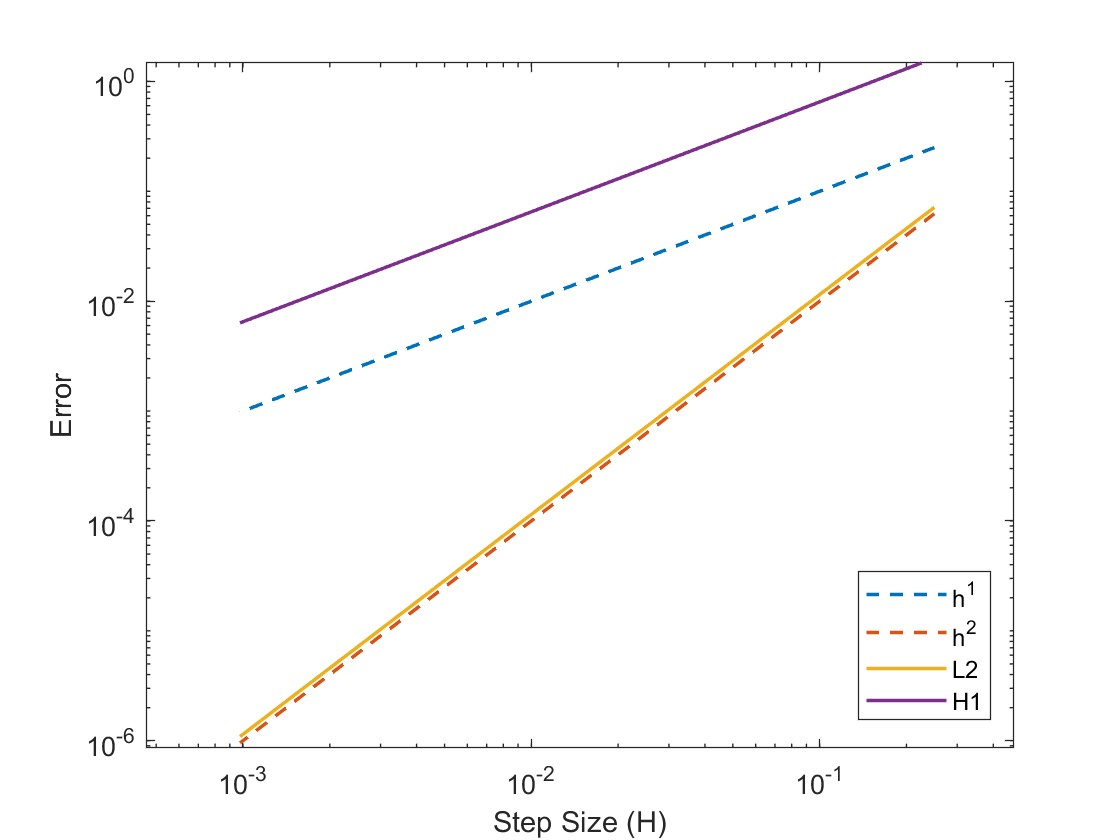
\includegraphics[width=\linewidth]{figures/dg_elliptic_uniform_mesh_exact_sol_errors_P1.jpg}
        \caption{Errors of SIPG for $P^1$-elements}
        \label{fig:elliptic_uniform_mesh_p1}
    \end{minipage}
    \hfill
    \begin{minipage}[t]{0.48\textwidth}
        \centering
        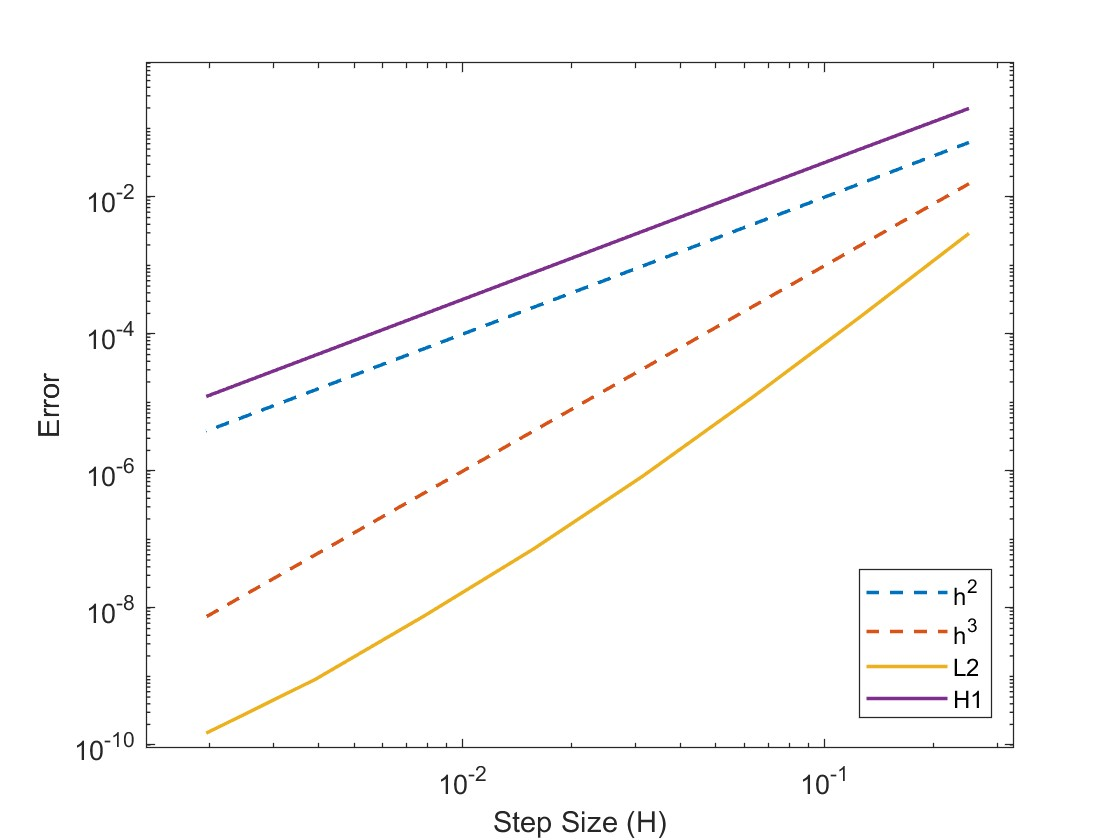
\includegraphics[width=\linewidth]{figures/dg_elliptic_uniform_mesh_exact_sol_errors_P2.jpg}
        \caption{Errors of SIPG for $P^2$-elements}
        \label{fig:elliptic_uniform_mesh_p2}
    \end{minipage}
\end{figure}

Finally we repeated the tests above using a non constant yet still smooth coefficient $c(x) = \sin(10x) + 2$ and observed no significant change in the results. 
To guarantee coercivity of the bilinear form we have to choose a slightly bigger $\sigma$ here.

